\section{Evaluation based on clustering and random forest.}\label{app:clustering}

The final method to evaluate the features importance in a strategy's success
is a combination of a clustering task and a random forest algorithm.
Initially the performances are clustered into different clusters
based on them being successful or not. The performances are clustered into
successful and unsuccessful clusters based on 4 different approaches.
More specifically:

\begin{itemize}
    \item \textbf{Approach 1:} The performances are divided into two clusters based
    on whether their performance was in the top \(5\%\) of their respective tournaments.
    Thus, whether \(r\) was smaller or larger than 0.05.
    \item \textbf{Approach 2:} The performances are divided into two clusters based
    on whether their performance was in the top \(25\%\) of their respective tournaments.
    Thus, whether \(r\) was smaller or larger than 0.25.
    \item \textbf{Approach 3:} The performances are divided into two clusters based
    on whether their performance was in the top \(50\%\) of their respective tournaments.
    Thus, whether \(r\) was smaller or larger than 0.50.
    \item \textbf{Approach 4:} The performances are clustered based on their normalised rank and
    their median score by a \(k-\)means algorithm~\cite{Arthur2007}. The number of
    clusters is not deterministically chosen but it is based on the silhouette
    coefficients~\cite{Rousseeuw1987}.
\end{itemize}

Once the performances have been assigned to a cluster for each approach a
random forest algorithm~\cite{breiman2001} is applied. The problem is a supervised
problem where the random forest algorithm predicts the cluster to which a performance
has been assigned to using the features of Table~\ref{table:manual_features}.
The random
forest models are trained on a training set of 70\% of the tournaments results.
The accuracy of each model based on $R^2$ and the number of clusters for each
tournament type (because in the case of Approach 4 it is not
deterministically chosen) are given by Table~\ref{table:accuracy_random_forest}.
The out of the bag error (OOB)~\cite{hastie2005} has also been calculated. The
models fit well, and a high value of both the accuracy measures on the test data
and the OOB error indicate that the model is not over fitting.

\begin{table}[!htbp]
    \begin{center}
        \resizebox{.9\textwidth}{!}{
        \begin{tabular}{lccccc}
    \toprule
    Tournament type & Clustering Approach & Number of clusters & $R^2$ training data &  $R^2$ test data  & $R^2$ OOB score\\
    \midrule
    standard  & Approach 1  & 2 & 0.998831  & 0.987041    & 0.983708 \\
              & Approach 2  & 2 & 0.998643  & 0.978626    & 0.969202 \\
              & Approach 3  & 2 & 0.998417  & 0.985217    & 0.976538 \\
              & Approach 4  & 2 & 0.998794  & 0.990677    & 0.982959 \\
    \midrule
    noisy     & Approach 1  & 2 & 0.997786  & 0.972229    & 0.968332\\
              & Approach 2  & 2 & 0.997442  & 0.963254    & 0.955219\\
              & Approach 3  & 2 & 0.997152  & 0.953164    & 0.940528\\
              & Approach 4  & 3 & 0.996923  & 0.950728    & 0.935444\\
    \midrule
    probabilistic ending & Approach 1 & 2 & 0.997909   & 0.981490  & 0.978120 \\
                         & Approach 2 & 2 & 0.997883   & 0.973492  & 0.967150 \\
                         & Approach 3 & 2 & 0.990448   & 0.890068  & 0.875822 \\
                         & Approach 4 & 2 & 0.999636   & 0.995183  & 0.992809 \\
    \midrule
    noisy probabilistic ending & Approach 1  & 2 & 0.995347 & 0.957846   & 0.952353\\
                               & Approach 2  & 2 & 0.992813 & 0.909346   & 0.898613\\
                               & Approach 3  & 2 & 0.990579 & 0.824794   & 0.806540\\
                               & Approach 4  & 4 & 0.989465 & 0.841652   & 0.824052\\
    \midrule
    over \numberofalltournaments tournaments   & Approach 1 & 2 & 0.997271& 0.972914& 0.969198 \\
                                               & Approach 2 & 2 & 0.996323& 0.951194& 0.940563 \\
                                               & Approach 3 & 2 & 0.993707& 0.906941& 0.891532 \\
                                               & Approach 4 & 3 & 0.993556& 0.913335& 0.898453 \\
    \bottomrule
        \end{tabular}}
    \end{center}
    \caption{Accuracy metrics for random forest models.}
    \label{table:accuracy_random_forest}
\end{table}

The importance that the features of Table~\ref{table:manual_features} had on
each random forest model are given by Figures~\ref{fig:clustering_importance_standard},
\ref{fig:clustering_importance_noise},~\ref{fig:clustering_importance_probend},
\ref{fig:clustering_importance_probend_noise}
and~\ref{fig:clustering_importance_overall}. These show that the classifiers
stochastic, make use of game and make use of length have no significant effect,
and several of the features that are highlighted by the importance are inline with
the correlation results. Moreover, the smoothing parameter \(k\) appears to no
have a significant effect either. The most important features based on the
random forest analysis were $C_{r} / C_{median}$ and $C_r / C_{mean}$.

\begin{figure}[!htbp]
    \begin{subfigure}[t]{0.5\textwidth}
        \begin{center}
            \includegraphics[width=.75\linewidth]{src/chapters/04/paper/meta-analysis-of-prisoners-dilemma-tournaments/new_output/standard/_feature_importance_bar_plot_cluster_on_0_05.pdf}
        \end{center}
        \caption{Importance of features for clusters on 5\% performance.}
    \end{subfigure}\hfill
    \begin{subfigure}[t]{0.5\textwidth}
        \begin{center}
            \includegraphics[width=.75\linewidth]{src/chapters/04/paper/meta-analysis-of-prisoners-dilemma-tournaments/new_output/standard/_feature_importance_bar_plot_cluster_on_0_25.pdf}
        \end{center}
        \caption{Importance of features for clusters on 25\% performance.}
    \end{subfigure}
    \begin{subfigure}[t]{0.5\textwidth}
        \begin{center}
            \includegraphics[width=.75\linewidth]{src/chapters/04/paper/meta-analysis-of-prisoners-dilemma-tournaments/new_output/standard/_feature_importance_bar_plot_cluster_on_0_5.pdf}
        \end{center}
        \caption{Importance of features for clusters on 50\% performance.}
    \end{subfigure}\hfill
    \begin{subfigure}[t]{0.5\textwidth}
        \begin{center}
            \includegraphics[width=.75\linewidth]{src/chapters/04/paper/meta-analysis-of-prisoners-dilemma-tournaments/k_means_output/standard/_feature_importance_bar_plot.pdf}
        \end{center}
        \caption{Importance of features for clusters based on \(k\)means algorithm.}
    \end{subfigure}
    \caption{Importance of features in standard tournaments for different
    clustering methods.}\label{fig:clustering_importance_standard}
\end{figure}

\begin{figure}[!htbp]
    \begin{subfigure}{0.5\textwidth}
        \begin{center}
            \includegraphics[width=.75\linewidth]{src/chapters/04/paper/meta-analysis-of-prisoners-dilemma-tournaments/new_output/noise/_feature_importance_bar_plot_cluster_on_0_05.pdf}
        \end{center}
        \caption{Importance of features for clusters on 5\% performance.}
    \end{subfigure}\hfill
    \begin{subfigure}{0.5\textwidth}
        \begin{center}
            \includegraphics[width=.75\linewidth]{src/chapters/04/paper/meta-analysis-of-prisoners-dilemma-tournaments/new_output/noise/_feature_importance_bar_plot_cluster_on_0_25.pdf}
        \end{center}
        \caption{Importance of features for clusters on 25\% performance.}
    \end{subfigure}
    \begin{subfigure}{0.5\textwidth}
        \begin{center}
            \includegraphics[width=.75\linewidth]{src/chapters/04/paper/meta-analysis-of-prisoners-dilemma-tournaments/new_output/noise/_feature_importance_bar_plot_cluster_on_0_5.pdf}
        \end{center}
        \caption{Importance of features for clusters on 50\% performance.}
    \end{subfigure}\hfill
    \begin{subfigure}{0.5\textwidth}
        \begin{center}
            \includegraphics[width=.75\linewidth]{src/chapters/04/paper/meta-analysis-of-prisoners-dilemma-tournaments/k_means_output/noise/_feature_importance_bar_plot.pdf}
        \end{center}
        \caption{Importance of features for clusters based on \(k\)means algorithm.}
    \end{subfigure}
    \caption{Importance of features in noisy tournaments for different
    clustering methods.}\label{fig:clustering_importance_noise}
\end{figure}

\begin{figure}[!htbp]
    \begin{subfigure}[t]{0.5\textwidth}
        \begin{center}
            \includegraphics[width=.75\linewidth]{src/chapters/04/paper/meta-analysis-of-prisoners-dilemma-tournaments/new_output/probend/_feature_importance_bar_plot_cluster_on_0_05.pdf}
        \end{center}
        \caption{Importance of features for clusters on 5\% performance.}
    \end{subfigure}
    \begin{subfigure}[t]{0.5\textwidth}
        \begin{center}
            \includegraphics[width=.75\linewidth]{src/chapters/04/paper/meta-analysis-of-prisoners-dilemma-tournaments/new_output/probend/_feature_importance_bar_plot_cluster_on_0_25.pdf}
        \end{center}
        \caption{Importance of features for clusters on 25\% performance.}
    \end{subfigure}
    \begin{subfigure}[t]{0.5\textwidth}
        \begin{center}
            \includegraphics[width=.75\linewidth]{src/chapters/04/paper/meta-analysis-of-prisoners-dilemma-tournaments/new_output/probend/_feature_importance_bar_plot_cluster_on_0_5.pdf}
        \end{center}
        \caption{Importance of features for clusters on 50\% performance.}
    \end{subfigure}
    \begin{subfigure}[t]{0.5\textwidth}
        \begin{center}
            \includegraphics[width=.75\linewidth]{src/chapters/04/paper/meta-analysis-of-prisoners-dilemma-tournaments/k_means_output/probend/_feature_importance_bar_plot.pdf}
        \end{center}
        \caption{Importance of features for clusters based on \(k\)means algorithm.}
    \end{subfigure}
    \caption{Importance of features in probabilistic ending tournaments for different
    clustering methods.}\label{fig:clustering_importance_probend}
\end{figure}

\begin{figure}[!htbp]
    \begin{subfigure}[t]{0.5\textwidth}
        \begin{center}
            \includegraphics[width=.75\linewidth]{src/chapters/04/paper/meta-analysis-of-prisoners-dilemma-tournaments/new_output/probend_noise/_feature_importance_bar_plot_cluster_on_0_05.pdf}
        \end{center}
        \caption{Importance of features for clusters on 5\% performance.}
    \end{subfigure}
    \begin{subfigure}[t]{0.5\textwidth}
        \begin{center}
            \includegraphics[width=.75\linewidth]{src/chapters/04/paper/meta-analysis-of-prisoners-dilemma-tournaments/new_output/probend_noise/_feature_importance_bar_plot_cluster_on_0_25.pdf}
        \end{center}
        \caption{Importance of features for clusters on 25\% performance.}
    \end{subfigure}
    \begin{subfigure}[t]{0.5\textwidth}
        \begin{center}
            \includegraphics[width=.75\linewidth]{src/chapters/04/paper/meta-analysis-of-prisoners-dilemma-tournaments/new_output/probend_noise/_feature_importance_bar_plot_cluster_on_0_5.pdf}
        \end{center}
        \caption{Importance of features for clusters on 50\% performance.}
    \end{subfigure}
    \begin{subfigure}[t]{0.5\textwidth}
        \begin{center}
            \includegraphics[width=.75\linewidth]{src/chapters/04/paper/meta-analysis-of-prisoners-dilemma-tournaments/k_means_output/probend_noise/_feature_importance_bar_plot.pdf}
        \end{center}
        \caption{Importance of features for clusters based on \(k\)means algorithm.}
    \end{subfigure}
    \caption{Importance of features in noisy probabilistic ending tournaments for different
    clustering methods.}\label{fig:clustering_importance_probend_noise}
\end{figure}

\begin{figure}[!htbp]
    \begin{subfigure}[t]{0.5\textwidth}
        \begin{center}
            \includegraphics[width=.75\linewidth]{src/chapters/04/paper/meta-analysis-of-prisoners-dilemma-tournaments/new_output/merged/_feature_importance_bar_plot_cluster_on_0_05.pdf}
        \end{center}
        \caption{Importance of features for clusters on 5\% performance.}
    \end{subfigure}
    \begin{subfigure}[t]{0.5\textwidth}
        \begin{center}
            \includegraphics[width=.75\linewidth]{src/chapters/04/paper/meta-analysis-of-prisoners-dilemma-tournaments/new_output/merged/_feature_importance_bar_plot_cluster_on_0_25.pdf}
        \end{center}
        \caption{Importance of features for clusters on 25\% performance.}
    \end{subfigure}
    \begin{subfigure}[t]{0.5\textwidth}
        \begin{center}
            \includegraphics[width=.75\linewidth]{src/chapters/04/paper/meta-analysis-of-prisoners-dilemma-tournaments/new_output/merged/_feature_importance_bar_plot_cluster_on_0_5.pdf}
        \end{center}
        \caption{Importance of features for clusters on 50\% performance.}
    \end{subfigure}
    \begin{subfigure}[t]{0.5\textwidth}
        \begin{center}
            \includegraphics[width=.75\linewidth]{src/chapters/04/paper/meta-analysis-of-prisoners-dilemma-tournaments/k_means_output/merged/_feature_importance_bar_plot.pdf}
        \end{center}
        \caption{Importance of features for clusters based on \(k\)means algorithm.}
    \end{subfigure}
    \caption{Importance of features over all the tournaments for different
    clustering methods.}\label{fig:clustering_importance_overall}
\end{figure}